\section{Bonus}
For changing the orbit blow equation must be true.

$$
r_1 = r_2 \to \dfrac{7200}{1+0.5\cos(\theta_1)} = \dfrac{8064}{1+0.2\cos(\theta_2)}
$$

Now we find $\theta_1$ respect to $\theta_2$.

$$
\theta_1 = \arccos\left((5\cos(\theta_2))/7 - 3/14\right)
$$

Now we make cost function.

$$
\text{Cost} = \left(\boldsymbol{v}_1 - \boldsymbol{v}_2\right)^2,~\boldsymbol{v}_1 
\begin{bmatrix}
    -\sin(\theta_1) & \cos(\theta_1)
\end{bmatrix},~\boldsymbol{v}_2 
\begin{bmatrix}
    -\sin(\theta_2) &
    \cos(\theta_2)
\end{bmatrix}
$$

Now we have a cost only function of $\theta_2$. Then, use fminbnd function of MATLAB to find minimum $\theta_2$.

$$
\min \theta_2 = -2.4189_{rad} = -138.6_{deg}
$$

\begin{figure}[H] 
    \caption{Cost in variation of $\theta_2$}
    \centering 
    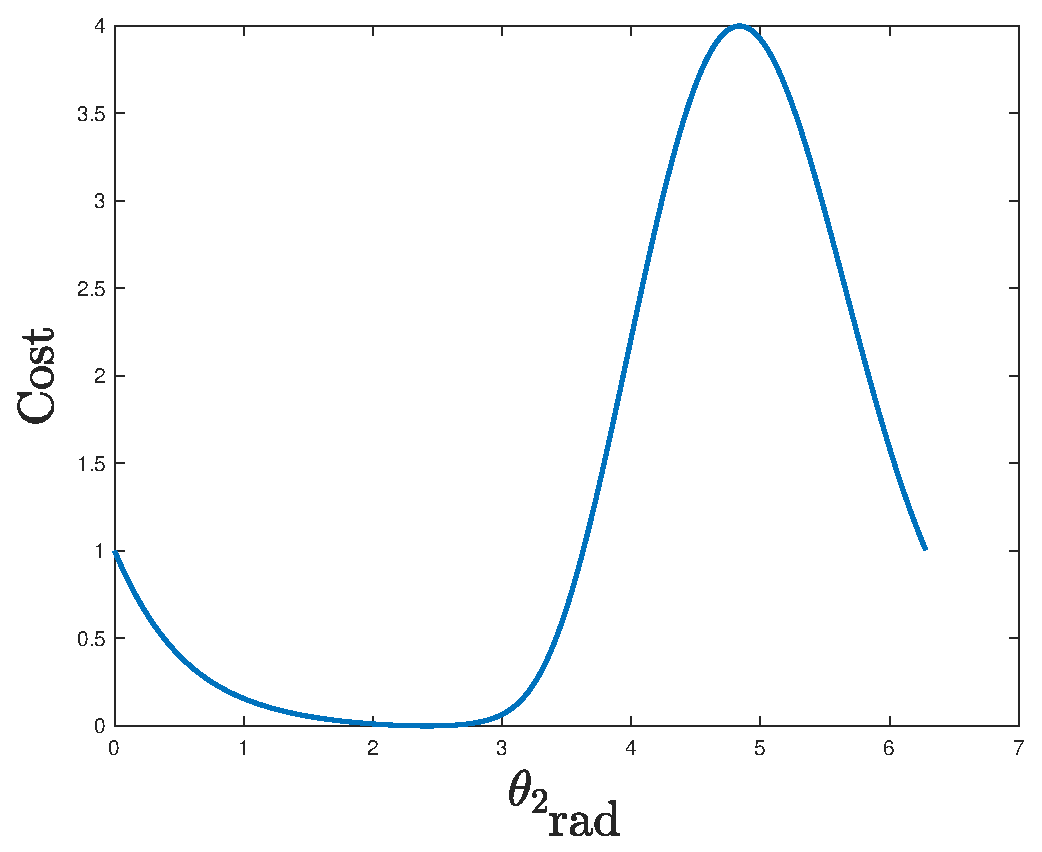
\includegraphics[width=12cm]{../Figure/Bonus/Cost} 
\end{figure}